\documentclass[12pt]{article}
\usepackage{graphicx}
\usepackage{latexsym, amsmath,amsfonts,amssymb}
\usepackage{xcolor}
\usepackage{fancyhdr}
\usepackage{fancybox}
\usepackage{nccmath}%to get small medium and large math
\usepackage{natbib,todonotes}
\usepackage{wrapfig}
\usepackage[margin=1in]{geometry}
\usepackage{kpfonts}  %Changing the default fonts
\usepackage[T1]{fontenc}
\usepackage{tkz-euclide}
\setlength{\parskip}{1.2ex} %space between paragraphs
\setlength{\parindent}{1em} %Paragraph indentation
\clubpenalty = 10000
\widowpenalty = 10000
\newcommand\T{\rule{0pt}{2ex}} % \T will create extra space above (used to fix tables)
\newcommand\B{\rule[-1.5ex]{0pt}{0pt}}% \B will create extra space below (used to fix tables)
\usetikzlibrary{calc,trees,positioning,arrows,chains,shapes.geometric,%
  decorations.pathreplacing,decorations.pathmorphing,shapes,%
  matrix,shapes.symbols,plotmarks,decorations.markings,shadows}
\linespread{1.25} %spacing between lines
\newtheorem{Theorem}{Theorem}
\pagestyle{empty}
\begin{document}
\begin{center}
\Large{\textbf{Thales' Theorem (3)}}
\end{center}
\textbf{Thales' Theorem:} If $A$, $B$, and $C$ are points on a circle and
$\overline{AB}$ is a diameter of the circle then $\angle \,ACB$ is a right angle.\\

\begin{center}
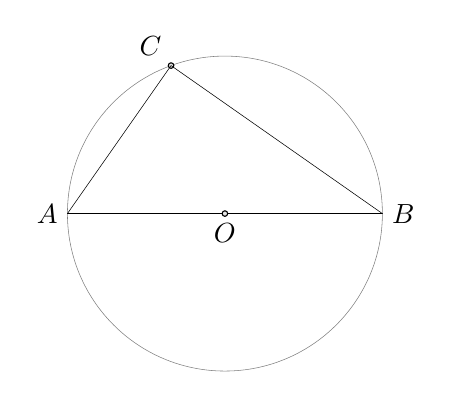
\begin{tikzpicture}[scale=2]
\tkzInit[xmin=-1.2,xmax=1.2,ymin=-1.2,ymax=1.2]
\tkzDefPoint(0,0){O}
\tkzDefPoint(1,0){B}
\tkzDefPoint(-1,0){A}
\tkzDrawCircle(O,A)
\tkzDrawSegment(A,B)
\tkzDefPoint(110:1){C}
\tkzDrawPoints(C,O)
\tkzDrawSegment(A,C)
\tkzDrawSegment(C,B)
\tkzLabelPoints[right](B)
\tkzLabelPoints[above left](C)
\tkzLabelPoints[left](A)
\tkzLabelPoints[below](O)
\end{tikzpicture}
\end{center}

\noindent\textbf{Proof:} Draw the figure in the coordinate plain. Let $O$ be the point $(0,0)$
and let $A$ and $B$ be the points $(-1,0)$ and $(1,0)$, respectively.

\begin{center}
\begin{tikzpicture}[scale=2]
\tkzInit[xmin=-1.2,xmax=1.2,ymin=-1.2,ymax=1.2]
\tkzDefPoint(0,0){O}
\tkzDefPoint(1,0){A}
\tkzDefPoint(-1,0){B}
\tkzDrawCircle(O,A)
\tkzDrawSegment(A,B)
\tkzDefPoint(110:1){C}
\tkzDrawPoints(C,O,A,B)
\tkzDrawSegment(A,C)
\tkzDrawSegment(C,B)
\tkzText(-1.35,0){$(-1,0)$}
\tkzText(1.3,0){$(1,0)$}
\tkzText(-.4,1.1){$(x,y)$}
\tkzText(0,-.2){$(0,0)$}
\end{tikzpicture}
\end{center}

The length of $\overline{AC}$ is $\sqrt{(x-(-1))^2 + (y-0)^2}=\sqrt{(x+1)^2 + y^2}$ and the 
length of $\overline{BC}$ is equal to $\sqrt{(x-(1))^2 + (y-0)^2}=\sqrt{(x-1)^2 + y^2}$. 
Finally, the length of $\overline{AB}$ is $\sqrt{(1-(-1))^2 + (0-0)^2}=\sqrt{(2)^2}=2$. Now
$(AC)^2 + (BC)^2 = \left((x+1)^2 + y^2\right) + \left((x-1)^2 + y^2\right) = x^2+2x+1+y^2 +
x^2-2x+1+y^2=2x^2+2y^2+2$ and since $(x,y)$ is on the unit circle, it follows that
$x^2+y^2=1$. This allows us to conclude $(AC)^2 + (BC)^2 = 2x^2+2y^2+2=2(x^2+y^2)+2=2(1)+2=4$.
Since  $(AB)^2=2^2=4$, the Pythagorean Theorem Converse allows us to conclude this triangle is
a right triangle and because the point $(x,y)$ is arbritrary, Thales' Theorem has been proven.
\end{document}